%\title{My two column CV}
%
% tccv (two columns curriculum vitae) is a LaTeX class inspired by
% the template found at latextemplates.com by Alessandro Plasmati.
%
% Create by Nicola Fontana, the original files can be downloaded from:
% http://dev.entidi.com/p/tccv/
%
\documentclass{tccv}
\usepackage[english]{babel}
\usepackage{graphicx}
\usepackage{placeins}

\begin{document}

\part{Michael. C. J. Kao}

\section{Personal Summary}

Highly skilled data scientist with hands-on knowledge of the latest
statistic and machine learning technique with a problem-solving
mindset at the core.\\

Proficient in R and Python for analysis and data preparation. Seasoned
in working with standard database and adept at scrapping unstructured
data from the web.\\

Strong business acumen and proven records of using analytics to
enhance business performance. 


%% Experienced in a plethora of statistical and machine learning
%% techniques from regression, classification, image processing, and
%% neural networks. Strong capacity of developing algorithm in both R and
%% Python to solve complex problems.\\

%% Expert in wrangling with data of any format, shape, and size, from
%% standard numerical data to texts and images. Experience working with
%% databases such as SQL and NoSQL, able to craft scraper or parser to
%% extract data from the web.\\

%% A skilled storyteller to communicate complex model and convey
%% intuition to the least technical audience.\\

%% I love diving, both in water and in data!


\section{Work experience}

\begin{eventlist}

\item{November 2016 -- July 2017}
  {Deepblu Inc, Taiwan}
  {Senior Data Scientist}

  Head the creation of the data team of a scuba diving social media
  startup.\\

  Laid the data infrastructure foundation, formulation of
  \textbf{expansion and retention strategy} and also \textbf{improved
    mobile app UX} with multiple custom algorithms .\\
 

\item{October 2011 -- Present}
  {FAO of the United Nations, Italy}
  {Lead Statistician}

  Lead the development of several flagship analytical projects
  including the latest Food Balance Sheet (FBS) for \textbf{monitoring
    global supply and demand of food} and ``The Reading Machine'' an AI
  program to decipher news article for \textbf{detection of food price
    anomalies}. \\

  %% The FBS project aggregates data from various sources, assisted with
  %% ensemble imputation provides a complete picture of supply and
  %% utilisation of agriculture products and the number of global
  %% undernourishment.\\

  %% The Reading Machine implements the state of art machine learning
  %% algorithm to harvest information in news articles to forecast
  %% agriculture commodity prices.


\item{June 2010 -- November 2011}
     {Ogilvy \& Mather, New Zealand}
     {Data Analyst}

     Analytical consultant delivering solutions to enhance decision
     making and business performance. Devised novel solutions to
     achieve goals from \textbf{increase return on media investment}
     to \textbf{provide statistical evidence for policy formulation}.


\end{eventlist}
%% \hspace{2in}

\begin{figure}%                 use [hb] only if necceccary!
  \centering
  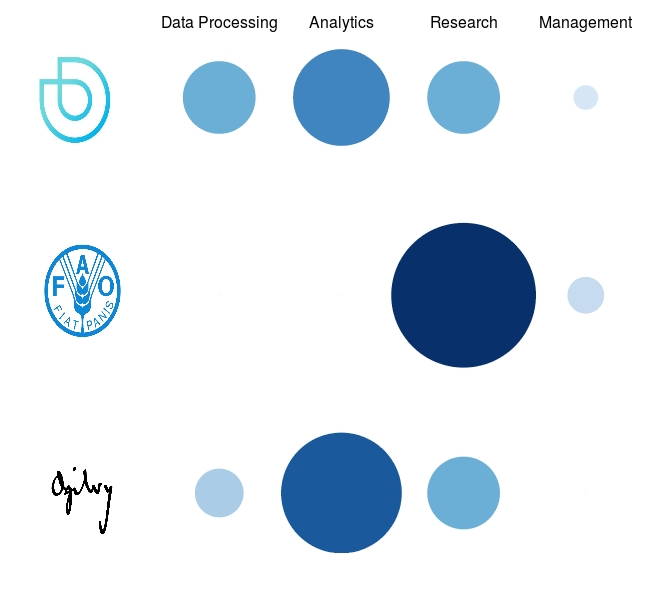
\includegraphics[width=9cm]{experience_association.jpeg}
\end{figure}


\section{Software Skills}
\begin{factlist}
\item{Languages}
  {R, Python and shell}
\item{Packages} {mlr, shiny, pandas, numpy, scipy, sciki-learn,
  tensorflow, airflow and django}
\item{Database}
  {*Sql, PostGIS, Mongo}
\item{Other}
     {Linux, Docker and Git}
\end{factlist}




\section{Education}

\begin{yearlist}

\item[University of Auckland]{2010 -- 2012}
     {M.Sc. in Statistic}
     %% {SNM-GARCH: A semi-parametric mixture extension to GARCH modelling}
{}

\item[University of Auckland]{2009 -- 2010}
     {B.A. (1st Class Hons.) \newline in Statistics}
     %% {Complex Demodulation/Remodulation of Electricity Consumption Time Series.}
{}

\item[University of Auckland]{2005 -- 2009}
  {B.A. \& B.Sc}
  {}
  %% {Majored in Economics, \newline Finance and Statistics}

%% \item[Coursera.org]{On-Going}
%%      {Online Course (MOOC)}
%%      {Machine Learning \newline Networked Life \newline Data Science}

%% \item[PADI \& TDI]{On-going}
%%   {Dive Master \newline Full Cave Diver \newline Extended Range}
%%      {}


%% \item[MOOC]{On-going}
%%   {Various Courses}
%%   {}

    
\end{yearlist}

%% \vspace{5in}
\section{Personal Info}

\begin{factlist}

\item{Email:}
  {mkao006@gmail.com}

\item{LinkedIn:}
  {\href{https://www.linkedin.com/in/mkao006/}{https://www.linkedin.com/in/mkao006/}}

\item{Github:}
  {\href{https://github.com/mkao006}{https://github.com/mkao006}}

\item{Nationality:}
  {New Zealand/Taiwan}

%% \item{Blog:}
%%      {\href{http://stateastics.com}{http://stateastics.com}}


\end{factlist}


%% \section{Awards \& Scholarships}

%% \begin{yearlist}

%% \item{2011}
%%      {RSVP and Nexus Award \newline for marketing insight}
%%      {}

%% \item{2011}
%%      {Master of Science Faculty Award with Scholarship}
%%      {}

%% \item{2010, 2011}
%%      {Senior Prize in Statistics}
%%      {}
          

%% \end{yearlist}












\vspace{5in}

\section{Selected Projects}
\begin{yearlist}

\item{2018} {Diamond Analysis} {Scrapped diamond data from James Allen
  to analyse and identify the best diamond to purchase for the
  engagement ring.}
  
\item{2017} {Automated Data pipeline} {Employed Airflow to automate
  and streamline the process of converting raw data into analytical
  products.}
  
\item{2017} {Dive Log Validation and Classification} {Implemented the
  isolation forest to detect anomalies in dive logs such as dive
  computer failure, incorrect air mixture, and infeasible profile to
  \textbf{improve the soundness and safety of diving}.}

\item{2016} {The Reading Machine
  (\href{https://github.com/EST-Team-Adam/TheReadingMachine}{Github})}
  {Automated forecasting of commodity price utilising information
    scrapped from web pages. Sentiment extraction and topic modeling
    of news article coupled with Recurrent Neural Network to forecast
    the commodity price. The purpose of the project is to
    \textbf{identify potential food crisis and provide lead time for
      reaction}.}
  
%% \item{2016} {DataKind Datadive Hackathon} {Prototyped a web app in
%%   Shiny to provide information on the animal density and observation
%%   trend.}
  
\item{2014} {Ensemble Imputation
  (\href{https://github.com/mkao006/sws\_imputation}{Github})} {Lead
  research on flexible and robust imputation methodology. An ensemble
  learning model was formulated to impute the global production of all
  agricultural products. \textbf{Over 200,000 time series were tested
    and imputed}.}

%% \item{2014} {Information Quality
%%   (\href{https://github.com/mkao006/sws\_flag}{Github})} {Use of
%%   entropy to measure relative information content of various data
%%   sources in order to \textbf{measure the quality of information} and
%%   construction of distribution for modelling.}

%% \item{2013}
%%      {Sentimental Mining
%%        (\href{https://github.com/mkao006/sofi\_twitter\_activity}{Github})}
%%      {Scrapped Twitter data for sentimental analysis in order to
%%        understand the reader response to flagship publication}

\item{2013}
     {R package: FAOSTAT
       (\href{http://cran.r-project.org/web/packages/FAOSTAT/index.html}{CRAN})}
     {An R package providing seamless integration to the FAO
       Statistics database.}

\item{2011} {Project 'KARMA'
  (\href{http://nzdmawards.co.nz/winners-archive/2011-winners-gallery/ministry-of-education-what-teacher-shortage}{RSVP
    Award})} {Forecasted demand and supply of teachers and analysed
  the labour force to provide insights on the reality of the teaching
  force. The RSVP and Nexus prize was awarded for \textbf{confirming
    that the teacher shortage was truly over and assisted in new
    policy formulation}.}

\end{yearlist}


\begin{yearlist}     
\item{2011} {Project 'MOA'} {The project estimated the effects of
  various advertising channel in order to assess the respective
  efficiency and effectiveness. The estimations were then employed to
  optimise the allocation of the marketing budget for a large retail
  banking client. The result was a \textbf{79\% improvement in
    customer acquisition over the existing budget}.}


\item{2011}
     {Campaign 'AND'}
     {The project identified segments of individuals which are high
       achievers from students of economically deprived
       background. The uses of the PRIM algorithm \textbf{pinpoint a
         segment with a 70\% completion rate as opposed to the pool
         average of 41\%}. This resulted in improved utilisation of
       public funding.}

\end{yearlist}

%% \section{Expertise and Skills}

%% \begin{itemize}
%%   \item Quantitative: Strong background in both theory and
%%     application. Experience in a broad range of statistical methods
%%     from time series, classification to machine learning and network
%%     analysis.

%%     \item Data handling: Ability to process and analyze data of any
%%       structure, satellite images, texts, sparse or large data.
      
%%     \item Problem Solving: Solution oriented, able to manage
%%       constraints and ability to communicate to solve the intended
%%       problem.
%% \end{itemize}


\begin{factlist}

\end{factlist}

\section{Language Proficiency}

\begin{factlist}
\item{English}{Native}
\item{Chinese}{Native}
\item{Taiwanese}{Native}
%% \item{Italian}{Conversational -- EU A1}
\item{Spanish}{Conversational -- EU A1}
\end{factlist}


\section{Interests}

\begin{factlist}
\item{Sports} {Scuba diving, basketball, boxing and bouldering}
%% \item{Hobbies} {Exploration}
\end{factlist}

\FloatBarrier
  \centering
  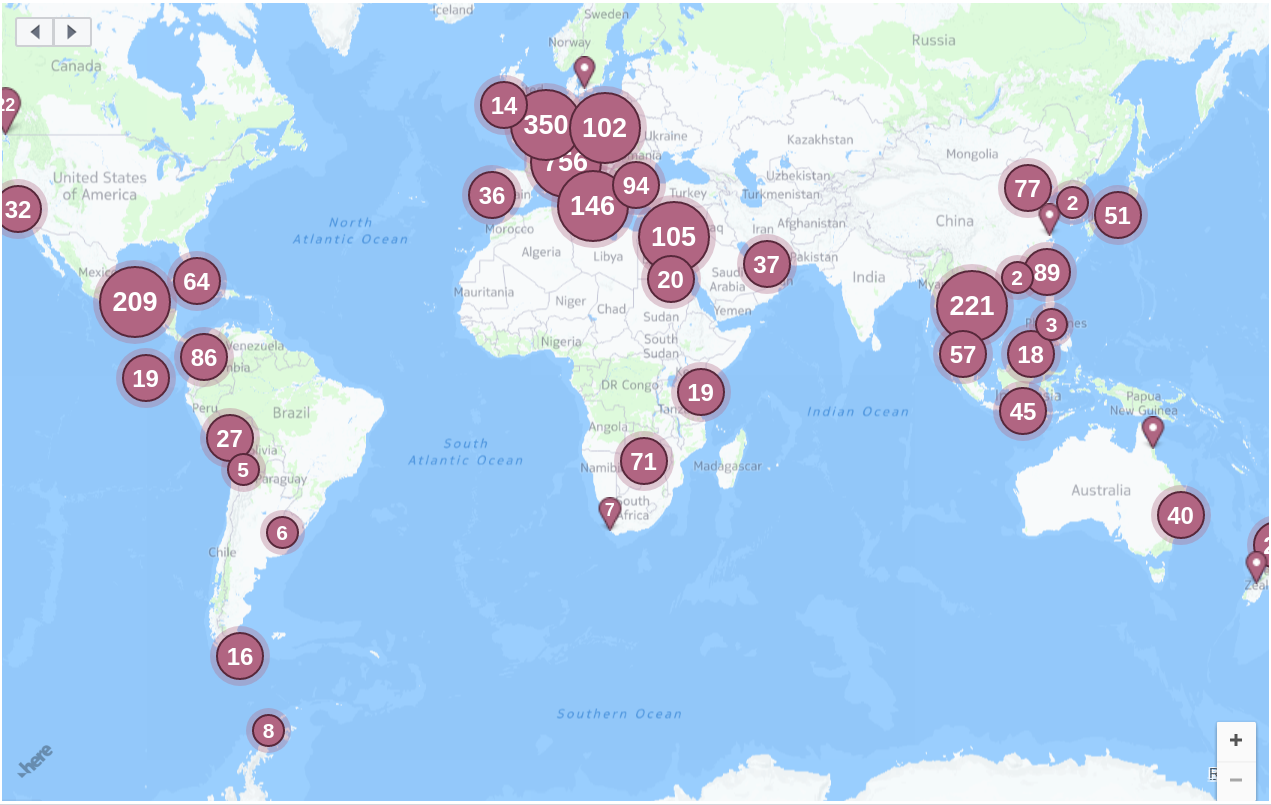
\includegraphics[scale = 0.2]{places_I_have_been_2.png}
  \textit{Places I have visited}
\FloatBarrier



\end{document}
